\chapter{Возможности оптимизации фазированных антенных решеток в различных условиях}\label{sec:radio}

\section{Исследование радиочастотных зависимостей}
 На практике использование высоко симметричных ФАР вызывает особый интерес из следующих соображений: измерение матрицы сопротивлений является тривиальной задачей, в то время как измерение парциальных полей требует большое количество приемников для всех возможных направлений излучения. Использование высокосимметричных ФАР позволяет выполнить расчеты для одного направления и затем легко адаптировать их для дугих симметричных направлений. Другой особенностью, влияющей на результаты моделирования является наличие потерь в земле (см.~\cite{yurkov:groundloss}). Чтобы ослабить этот эффект, антенные системы с противовесами подняты над землей на 2м.

В данной главе изучается, как изменяется общий коэффициент усиления с ростом радиочастоты и плотности системы противовесов. Общий коэффициент усиления является суммой частичных коэффициентов усиления в  двух ортогональных поляризациях. Плотность системы противовесов определяется числом продольных и поперечных проводов, относящихся к одному и тому же излучателю. Частота изменяется от 5 до 30 МГц. Вычисления производились на решетках ШВИ, состоящих из 8 излучателей. Для расчета матрицы сопротивлений и матрицы излучений использовался пакет моделирования антенных систем NEC2~\cite{bruke:nec2}.

Для проведения вычислительного эксперимента использовался решатель BARON в пакете GAMS. Результаты оптимизации направленности решетки сравниваются с коэффициентом усиления одиночного излучателя, установленного в центре такой же системы противовесов. Плотность системы противовесов обозначается в формате $long:trans$, где $long$ - число продольных проводов, относящихся к одному излучателю, а $trans$ - поперечных. Высота каждого ШВИ - 15м. В качестве направления оптимизации выбирается $70^{\circ}$ полярного угла и $45^{\circ}$ азимутального угла в сферических координатах.

\begin{figure}
\center{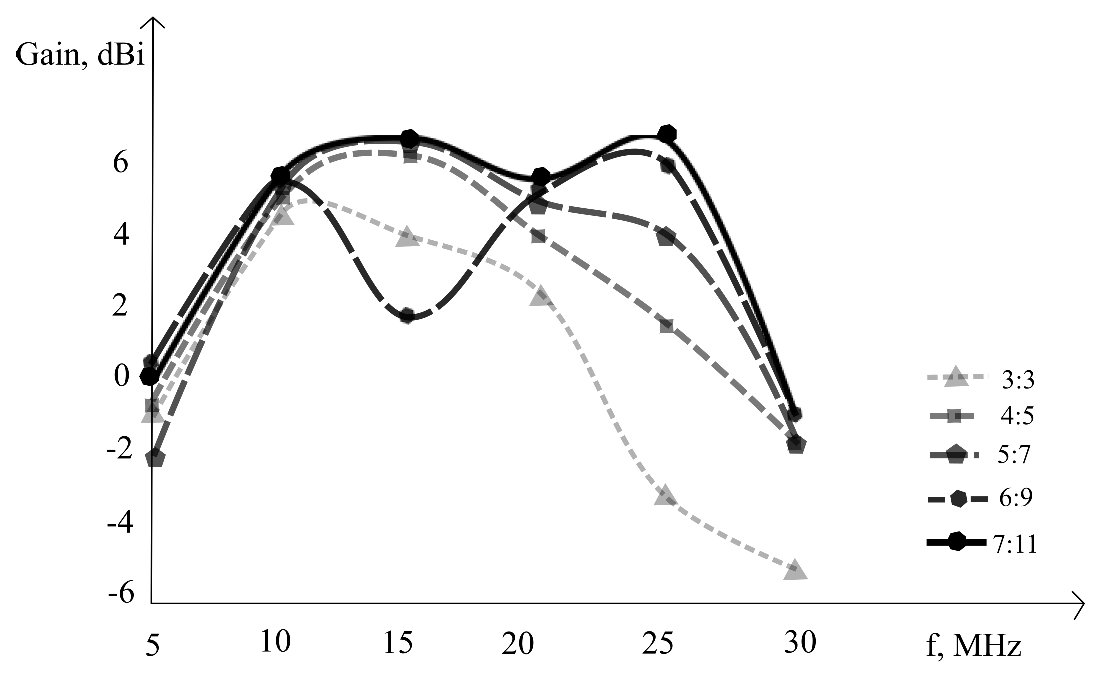
\includegraphics[width=0.8\linewidth]{ring_f__paa_gains.eps}}
\caption{Зависимость от частоты общего коэффициента усиления ФАР при оптимизации в направлении 70:45}
\label{ris:paa_gains}
\end{figure}

На рис.~\ref{ris:paa_gains} показано, как изменяется коэффициент усиления с ростом радиочастоты. Можно наблюдать, что при крайних значениях частоты 5 и 30 МГц решетка малоэффективна. Также можно увидеть, что, в основном, увеличение плотности системы противовесов приводит к росту коэффициента усиления. Единственное исключение - решетка с плотностью системы противовесов $6:9$ на частоте 15МГц, где наблюдается неожиданное падение коэффициента усиления. Такое поведение может быть объяснено тем, что BARON не достиг глобалного оптимума.

\begin{figure}
\center{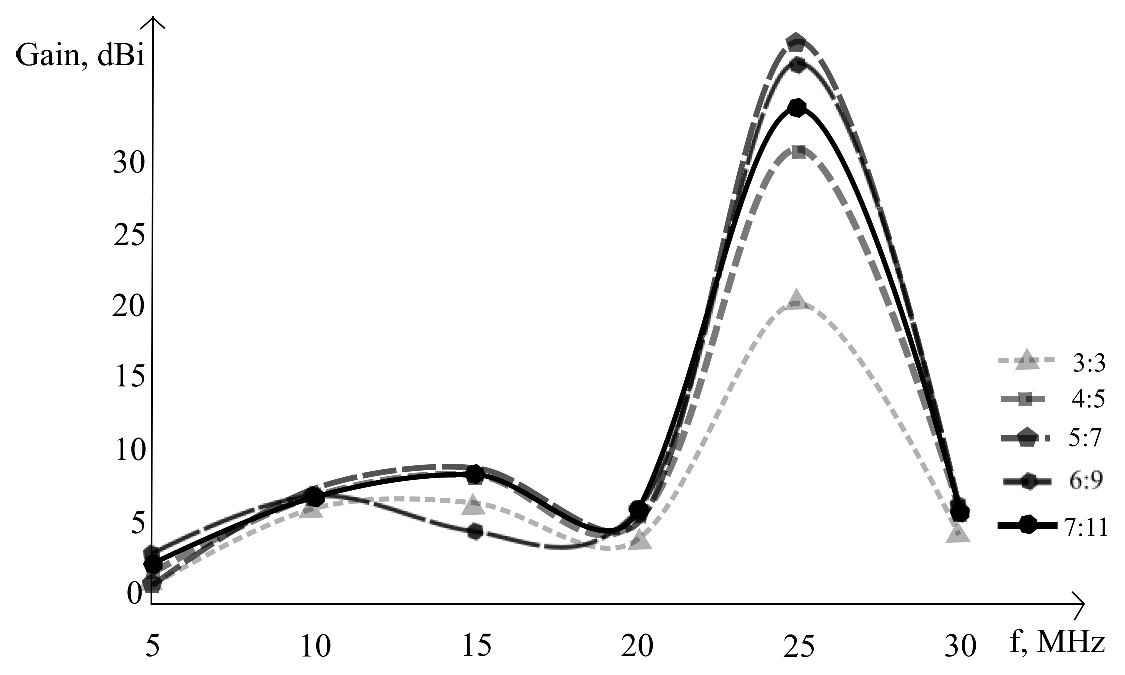
\includegraphics[width=0.8\linewidth]{ring_f_gains.eps}}
\caption{Сравнение коэффициентов усиления ФАР и одиночного излучателя}
\label{ris:all_gains}
\end{figure}

На рис.~\ref{ris:all_gains} показано, как изменяется соотношение коэффициентов усиления ФАР и одиночного излучателя с ростом частоты. Заметным результатом здесь является то, что на частоте 25МГц усиление ФАР существенно больше усиления одиночного излучателя. Объяснение этого эфффекта будет приведено далее при сравнении диаграмм направленности. При 5МГц усиление ФАР существенно не превосходит усиление одиночного излучателя, однако, уже на 10МГц разница возрастает до 7.53дБ. Даже при 30МГц, где ФАР малоэффективна, разница с одиночным излучателем составляет 6.63дБ в лучшем случае и 4.84дБ в худшем.

Далее будут рассмотрены диаграммы направленности ФАР с плотностью противовесов $5:7$ как один из наиболее типичных результатов.

\begin{figure}
\begin{minipage}[h]{0.49\linewidth}
\center{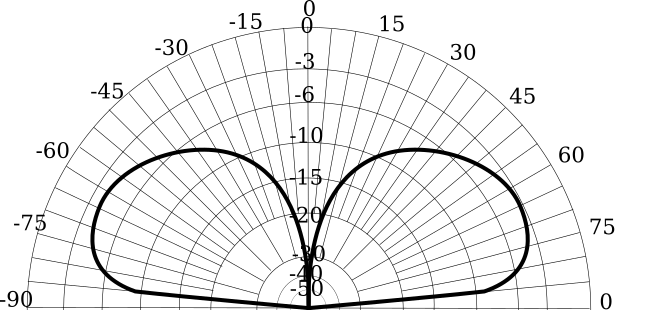
\includegraphics[width=1\linewidth]{r8_1_5_5x7.png} \\ a)}
\end{minipage}
\hfill
\begin{minipage}[h]{0.49\linewidth}
\center{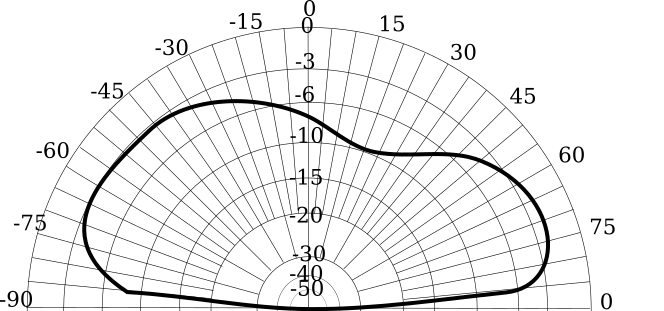
\includegraphics[width=1\linewidth]{r8_5_5x7.png} \\ b)}
\end{minipage}
\caption{Вертикальный план диаграммы направленности одиночного излучателя (a) и ФАР 5:7 (b) при 5МГц}
\label{ris:5MHz}
\end{figure}

При частоте 5МГц (см. рис.~\ref{ris:5MHz}) мы можем наблюдать, что максимум усиления в случае ФАР приходится на $70^{\circ}$ и превосходит соответствующее значение одиночного излучателя на 1.33~дБ. Использование ФАР с плотностью системы противовесов 6:9 позволяет увеличить этот параметр до 3.14~дБ.

\begin{figure}
\begin{minipage}[h]{0.49\linewidth}
\center{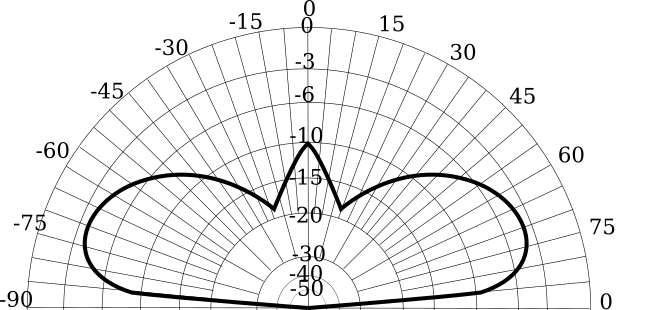
\includegraphics[width=1\linewidth]{r8_1_10_5x7.png} \\ a)}
\end{minipage}
\hfill
\begin{minipage}[h]{0.49\linewidth}
\center{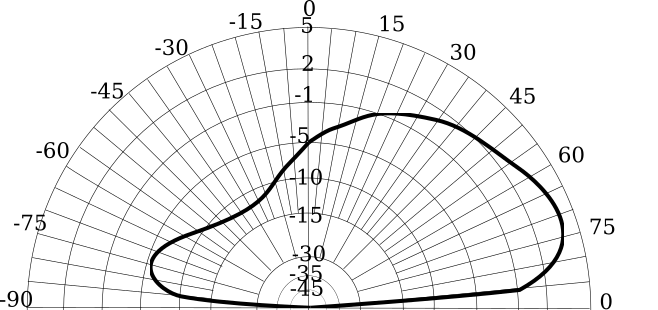
\includegraphics[width=1\linewidth]{r8_10_5x7.png} \\ b)}
\end{minipage}
\caption{Вертикальный план диаграммы направленности одиночного излучателя (a) и ФАР 5:7 (b) при 10МГц}
\label{ris:10MHz}
\end{figure}

Результат оптимизации более заметен при частоте 10МГц~(см~Рис.~\ref{ris:10MHz}): задний лепесток существенно меньше и разница усиления к одиночному излучателю достигает примерно~8~дБ. Похожие результаты наблюдаются при частоте~15МГц.

\begin{figure}
\begin{minipage}[h]{0.49\linewidth}
\center{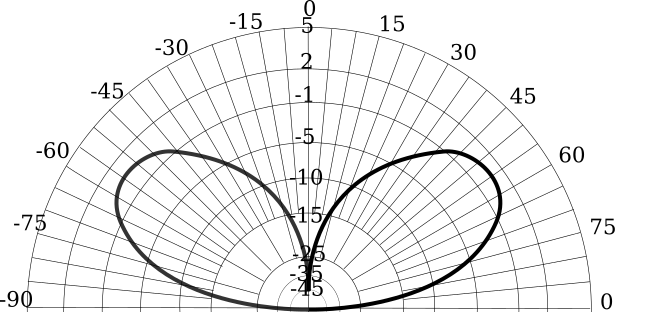
\includegraphics[width=1\linewidth]{r8_1_20_5x7.png} \\ a)}
\end{minipage}
\hfill
\begin{minipage}[h]{0.49\linewidth}
\center{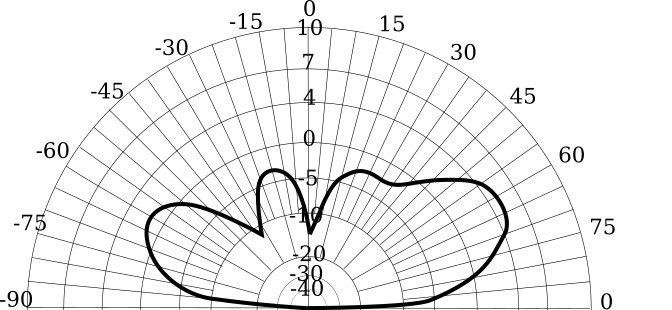
\includegraphics[width=1\linewidth]{r8_20_5x7.png} \\ b)}
\end{minipage}
\caption{Вертикальный план диаграммы направленности одиночного излучателя (a) и ФАР 5:7 (b) при 20МГц}
\label{ris:f20mhs}
\end{figure}

При 20МГц можно наблюдать, что как в случае одиночного излучателя, так и в случае ФАР, коэффициент усиления падает по отношению к результату при 15МГц~(см~Рис.~\ref{ris:paa_gains}). Диаграмма направленности изображена на рис.~\ref{ris:f20mhs}.

\begin{figure}
\begin{minipage}[h]{0.49\linewidth}
\center{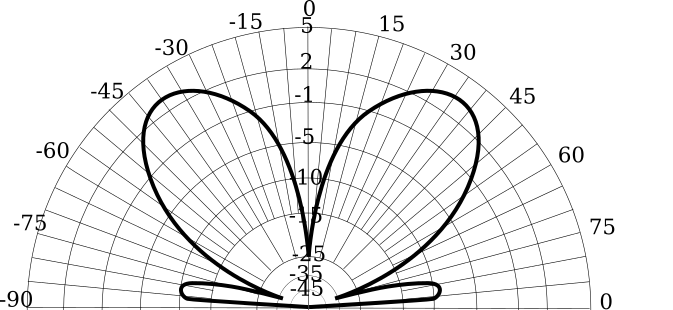
\includegraphics[width=1\linewidth]{r8_1_25_5x7.png} \\ a)}
\end{minipage}
\hfill
\begin{minipage}[h]{0.49\linewidth}
\center{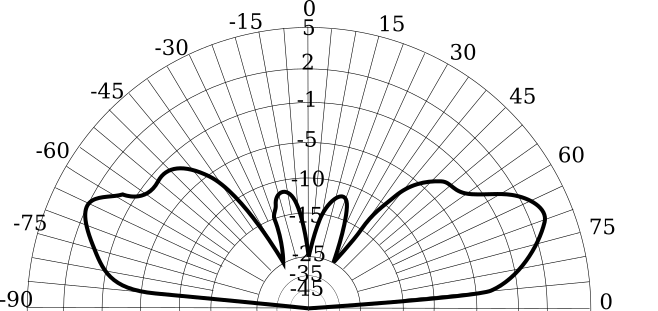
\includegraphics[width=1\linewidth]{r8_25_5x7.png} \\ b)}
\end{minipage}
\caption{Вертикальный план диаграммы направленности одиночного излучателя (a) и ФАР 5:7 (b) при 25МГц}
\label{ris:f25mhs}
\end{figure}

Интересный результат наблюдается при 25МГц (см~Рис.~\ref{ris:f25mhs}), где усиление ФАР существенно больше усиления одиночного излучателя. Сравнение их диаграмм направленности показывает, что одиночный излучатель мало излучает в направлении оптимизации, тогда как ФАР имеет максимум излучения в этом направлении. Невозможно было бы достигнуть такого явления без учета взаимного влияния. Отсюда следует, что при оптимизации направленности ФАР КВ диапазона не следует пренебрегать взаимным влиянием, поскольку это может существенно изменить вид диаграммы направленности.

Далее рассмотрим как горизонтальный план диаграммы направленности меняется с ростом частоты~(см. рис.~\ref{ris:horizontal}). Направление оптимизации - $45^{\circ}$. Здесь мы можем наблюдать, что при частоте, равной 5МГц, диаграмма направленности представляется почти овальной формой. Дальнейшее увеличение частоты до 15МГц приводит диаграмму направленности к направленной форме. Затем увеличение частоты ведет к довольно сложной форме, при которой максимум излучения становится менее ярко выражен.

\begin{figure}
\begin{minipage}[h]{0.49\linewidth}
\center{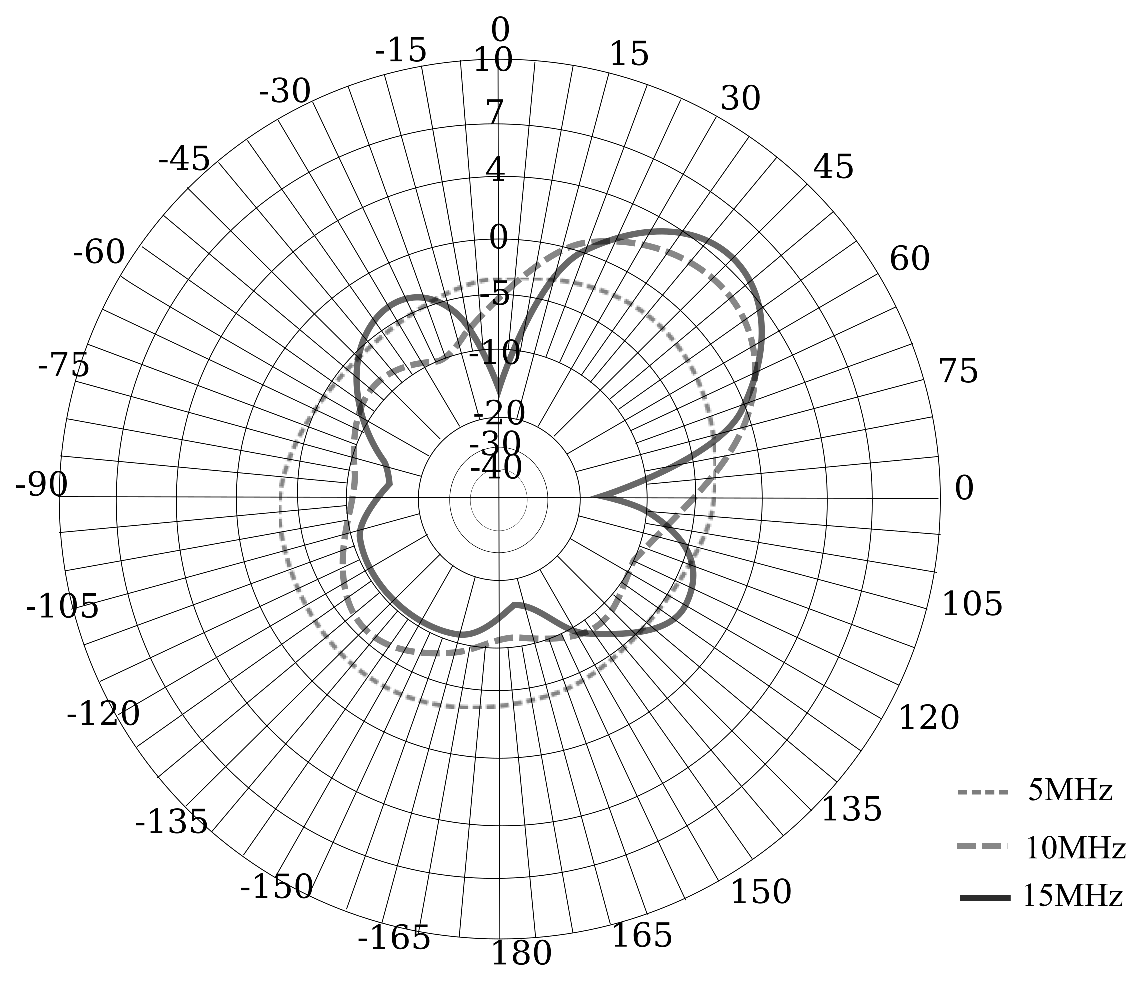
\includegraphics[width=1\linewidth]{r8_horizontal_5x7.eps} \\ a)}
\end{minipage}
\hfill
\begin{minipage}[h]{0.49\linewidth}
\center{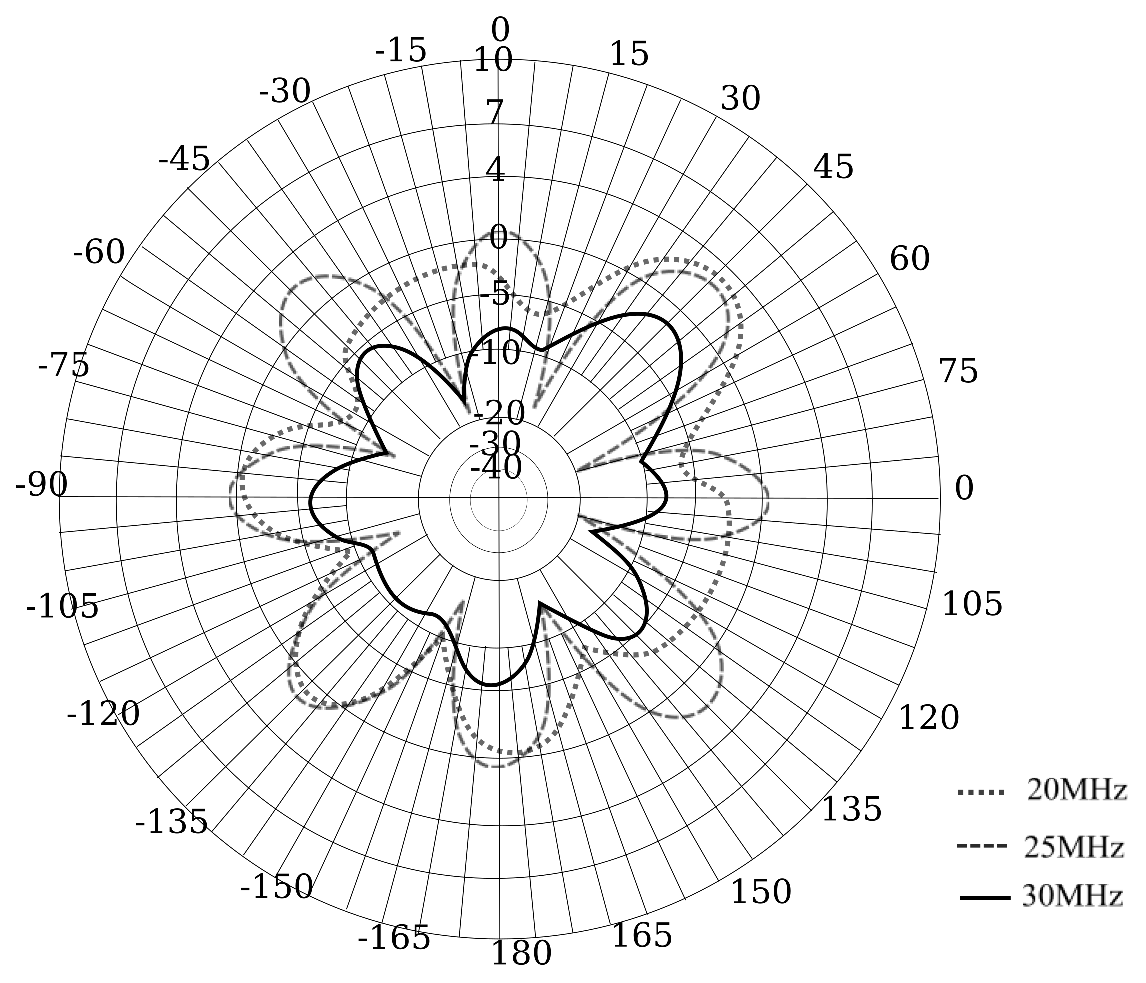
\includegraphics[width=1\linewidth]{r8_horizontal_5x7_2.eps} \\ b)}
\end{minipage}
\caption{Горизонтальный план диаграммы направленности для ФАР 5:7 5-15МГц (a) и 20-30МГц (b)}
\label{ris:horizontal}
\end{figure}

\section{Исследование взаимного влияния излучателей}

Все эксперименты проводились при реальной земле, рассчитанной по методу Зоммерфельда-Нортона пакетом NEC-2. Для проведения эксперимента было выбрано несколько частот в рабочем диапазоне, однако, все приведенные в данной статье результаты приходятся на 5 МГц, поскольку именно эти результаты носят наиболее иллюстративный характер.
Рассмотрим случай фазирования решетки без учета взаимного влияния ее элементов. Для этого обратимся к формуле~(\ref{eq:A}). Если пренебречь взаимным влиянием излучателей, плотность мощности $F$ будет максимальна тогда, когда комплексные амплитуды парциальных полей будут синфазны. В данной главе производилось сравнение диаграмм направленности решеток разных конфигураций после математической оптимизации их направленности в заданном направлении согласно модели~(\ref{eq:task3}) с соответствующими диаграммами одиночного излучателя и со случаем фазирования решетки без учета взаимного влияния (далее – простое фазирование).
Для проведения вычислительного эксперимента использовался решатель BARON в пакете GAMS, поскольку, как правило, он обеспечивает бо́льшую точность решений по сравнению с градиентным подъемом. Высота каждого ШВИ равна 15 м. Длина плеча симметричных излучателей также равна 15м.
Каждая кольцевая решетка состоит из восьми излучателей. Направление оптимизации по умолчанию было установлено на $70^{\circ}$ полярного угла и $45^\circ$ азимутального угла в сферических координатах. Для некоторых экспериментов было проведено дополнительное исследование при $85^\circ$ полярного угла.


\subsection{Широкополосные вертикальные излучатели}
В рамках данного эксперимента производилось сравнение диаграмм направленности при варьировании расстояния центра излучателя до центра решетки (от 7 до 80м), длины радиальных противовесов (от 3 до 20м) и присутствия или отсутствия общей системы противовесов. Диаграммы направленности при этом имели различную форму, однако, качественно различие между коэффициентами усиления всегда сохранялось (см.~рис.~\ref{ris:bve_mut_5_8}): результат оптимизации не давал значимого преимущества перед простым фазированием.  Модули диагональных и недиагональных элементов матрицы проводимостей в указанном примере не превосходили 0.002 и 0.0003 См соответственно.

\begin{figure}
\begin{minipage}[h]{0.49\linewidth}
\center{\includegraphics[width=1\linewidth]{mut/bve/5/8/h.eps} \\ a)}
\end{minipage}
\hfill
\begin{minipage}[h]{0.49\linewidth}
\center{\includegraphics[width=1\linewidth]{mut/bve/5/8/v.eps} \\ b)}
\end{minipage}
\caption{Горизонтальная (a) и вертикальная (b) плоскость диаграммы направленности ШВИ при расстоянии от центра излучателя до центра решетки 8м и длине радиальных противовесов 5м. Пунктирной линией обозначено усиление одиночного излучателя, штрихпунктирной -- простое фазирование, сплошной -- решение задачи мат. программирования.}
\label{ris:bve_mut_5_8}
\end{figure}

\begin{figure}
\begin{minipage}[h]{0.49\linewidth}
\center{\includegraphics[width=1\linewidth]{mut/bve/5/15/h.eps} \\ a)}
\end{minipage}
\hfill
\begin{minipage}[h]{0.49\linewidth}
\center{\includegraphics[width=1\linewidth]{mut/bve/5/15/v.eps} \\ b)}
\end{minipage}
\caption{Горизонтальная (a) и вертикальная (b) плоскость диаграммы направленности ШВИ при расстоянии от центра излучателя до центра решетки 15м и длиной радиальных противовесов 5м. Пунктирной линией обозначено усиление одиночного излучателя, штрихпунктирной -- простое фазирование, сплошной -- решение задачи мат. программирования.}
\label{ris:bve_mut_5_15}
\end{figure}

\subsection{Широкополосные вертикальные диполи}

Для ШВД производилось исследование диаграмм направленности при варьировании расстояния центра излучателя до центра решетки от 5 до 50м. В большинстве случаев, использование решения задачи математического программирования не давало существенного преимущества перед простым фазированием (см.~рис.~\ref{ris:ris:bvd_mut_5_10}). Модули диагонального и недиагонального элементов матрицы проводимостей в приведенном примере не превосходили 0.016 и 0.006 См соответственно.  Тем не менее, при расстоянии между центром излучателя и центром решетки равным 20м это различие составило около 4 дБ (см.~рис.~\ref{ris:ris:bvd_mut_5_20}). Здесь модули диагональных и недиагональных элементов матрицы проводимостей не превосходили 0.013 и 0.008См соответственно.

\begin{figure}
\begin{minipage}[h]{0.49\linewidth}
\center{\includegraphics[width=1\linewidth]{mut/bvd/5/10/h.eps} \\ a)}
\end{minipage}
\hfill
\begin{minipage}[h]{0.49\linewidth}
\center{\includegraphics[width=1\linewidth]{mut/bvd/5/10/v.eps} \\ b)}
\end{minipage}
\caption{Горизонтальная (a) и вертикальная (b) плоскость диаграммы направленности ШВД при расстоянии от центра излучателя до центра решетки 10м при частоте 5МГц. Пунктирной линией обозначено усиление одиночного излучателя, штрихпунктирной -- простое фазирование, сплошной -- решение задачи мат. программирования.}
\label{ris:bvd_mut_5_10}
\end{figure}

\begin{figure}
\begin{minipage}[h]{0.49\linewidth}
\center{\includegraphics[width=1\linewidth]{mut/bvd/5/50/h.eps} \\ a)}
\end{minipage}
\hfill
\begin{minipage}[h]{0.49\linewidth}
\center{\includegraphics[width=1\linewidth]{mut/bvd/5/50/v.eps} \\ b)}
\end{minipage}
\caption{Горизонтальная (a) и вертикальная (b) плоскость диаграммы направленности ШВД при расстоянии от центра излучателя до центра решетки 50м при частоте 5МГц. Пунктирной линией обозначено усиление одиночного излучателя, штрихпунктирной -- простое фазирование, сплошной -- решение задачи мат. программирования.}
\label{ris:bvd_mut_5_50}
\end{figure}


\begin{figure}
\begin{minipage}[h]{0.49\linewidth}
\center{\includegraphics[width=1\linewidth]{mut/bvd/5/20/h.eps} \\ a)}
\end{minipage}
\hfill
\begin{minipage}[h]{0.49\linewidth}
\center{\includegraphics[width=1\linewidth]{mut/bvd/5/20/v.eps} \\ b)}
\end{minipage}
\caption{Горизонтальная (a) и вертикальная (b) плоскость диаграммы направленности ШВД при расстоянии от центра излучателя до центра решетки 20м при частоте 5МГц. Пунктирной линией обозначено усиление одиночного излучателя, штрихпунктирной -- простое фазирование, сплошной -- решение задачи мат. программирования.}
\label{ris:bvd_mut_5_20}
\end{figure}

Также была произведена серия экспериментов при частоте 25МГц, однако, существенных преимуществ обнаружено не было (см.~рис.~\ref{ris:bvd_mut_25_10}).

\begin{figure}
\begin{minipage}[h]{0.49\linewidth}
\center{\includegraphics[width=1\linewidth]{mut/bvd/25/10/h.eps} \\ a)}
\end{minipage}
\hfill
\begin{minipage}[h]{0.49\linewidth}
\center{\includegraphics[width=1\linewidth]{mut/bvd/25/10/v.eps} \\ b)}
\end{minipage}
\caption{Горизонтальная (a) и вертикальная (b) плоскость диаграммы направленности ШВД при расстоянии от центра излучателя до центра решетки 10м при частоте 25МГц. Пунктирной линией обозначено усиление одиночного излучателя, штрихпунктирной -- простое фазирование, сплошной -- решение задачи мат. программирования.}
\label{ris:bvd_mut_25_10}
\end{figure}

\subsection{Симметричные вертикальные диполи}

Для решетки СВД при оптимизации в направлении полярного угла равном $70^{\circ}$ при варьировании расстояния от центра излучателя до центра решетки от 35 до 37м разница между коэффициентом усиления решения задачи математического программирования и усилением простого фазирования также достигала 4дБ. При этом модули диагональных и недиагональных элементов матрицы проводимостей не превосходили 0.033 и 0.021См соответственно.

\begin{figure}
\begin{minipage}[h]{0.49\linewidth}
\center{\includegraphics[width=1\linewidth]{mut/svd/5/70/15/h.eps} \\ a)}
\end{minipage}
\hfill
\begin{minipage}[h]{0.49\linewidth}
\center{\includegraphics[width=1\linewidth]{mut/svd/5/70/15/v.eps} \\ b)}
\end{minipage}
\caption{Горизонтальная (a) и вертикальная (b) плоскость диаграммы направленности СВД при расстоянии от центра излучателя до центра решетки 15м при оптимизации в направлении $70^{\circ}$ полярного угла. Пунктирной линией обозначено усиление одиночного излучателя, штрихпунктирной -- простое фазирование, сплошной -- решение задачи мат. программирования.}
\label{ris:svd_mut_5_70_15}
\end{figure}

\begin{figure}
\begin{minipage}[h]{0.49\linewidth}
\center{\includegraphics[width=1\linewidth]{mut/svd/5/70/25/h.eps} \\ a)}
\end{minipage}
\hfill
\begin{minipage}[h]{0.49\linewidth}
\center{\includegraphics[width=1\linewidth]{mut/svd/5/70/25/v.eps} \\ b)}
\end{minipage}
\caption{Горизонтальная (a) и вертикальная (b) плоскость диаграммы направленности СВД при расстоянии от центра излучателя до центра решетки 25м при оптимизации в направлении $70^{\circ}$ полярного угла. Пунктирной линией обозначено усиление одиночного излучателя, штрихпунктирной -- простое фазирование, сплошной -- решение задачи мат. программирования.}
\label{ris:svd_mut_5_70_25}
\end{figure}

\begin{figure}
\begin{minipage}[h]{0.49\linewidth}
\center{\includegraphics[width=1\linewidth]{mut/svd/5/70/27/h.eps} \\ a)}
\end{minipage}
\hfill
\begin{minipage}[h]{0.49\linewidth}
\center{\includegraphics[width=1\linewidth]{mut/svd/5/70/27/v.eps} \\ b)}
\end{minipage}
\caption{Горизонтальная (a) и вертикальная (b) плоскость диаграммы направленности СВД при расстоянии от центра излучателя до центра решетки 27м при оптимизации в направлении $70^{\circ}$ полярного угла. Пунктирной линией обозначено усиление одиночного излучателя, штрихпунктирной -- простое фазирование, сплошной -- решение задачи мат. программирования.}
\label{ris:svd_mut_5_70_27}
\end{figure}

\begin{figure}
\begin{minipage}[h]{0.49\linewidth}
\center{\includegraphics[width=1\linewidth]{mut/svd/5/70/35/h.eps} \\ a)}
\end{minipage}
\hfill
\begin{minipage}[h]{0.49\linewidth}
\center{\includegraphics[width=1\linewidth]{mut/svd/5/70/35/v.eps} \\ b)}
\end{minipage}
\caption{Горизонтальная (a) и вертикальная (b) плоскость диаграммы направленности СВД при расстоянии от центра излучателя до центра решетки 35м при оптимизации в направлении $70^{\circ}$ полярного угла. Пунктирной линией обозначено усиление одиночного излучателя, штрихпунктирной -- простое фазирование, сплошной -- решение задачи мат. программирования.}
\label{ris:svd_mut_5_70_35}
\end{figure}

\begin{figure}
\begin{minipage}[h]{0.49\linewidth}
\center{\includegraphics[width=1\linewidth]{mut/svd/5/70/40/h.eps} \\ a)}
\end{minipage}
\hfill
\begin{minipage}[h]{0.49\linewidth}
\center{\includegraphics[width=1\linewidth]{mut/svd/5/70/40/v.eps} \\ b)}
\end{minipage}
\caption{Горизонтальная (a) и вертикальная (b) плоскость диаграммы направленности СВД при расстоянии от центра излучателя до центра решетки 40м при оптимизации в направлении $70^{\circ}$ полярного угла. Пунктирной линией обозначено усиление одиночного излучателя, штрихпунктирной -- простое фазирование, сплошной -- решение задачи мат. программирования.}
\label{ris:svd_mut_5_70_40}
\end{figure}

При оптимизации в направлении полярного угла равном $85^{\circ}$ при варьировании расстояния от центра излучателя до центра решетки от 25 до 29м эта разница достигала 5дБ.~(см.~рис.~\ref{ris:svd_mut_5_85_25}). Здесь модули диагональных и недиагональных элементов матрицы проводимостей не превосходили 0.015 и 0.009См соответственно.

\begin{figure}
\begin{minipage}[h]{0.49\linewidth}
\center{\includegraphics[width=1\linewidth]{mut/svd/5/85/25/h.eps} \\ a)}
\end{minipage}
\hfill
\begin{minipage}[h]{0.49\linewidth}
\center{\includegraphics[width=1\linewidth]{mut/svd/5/85/25/v.eps} \\ b)}
\end{minipage}
\caption{Горизонтальная (a) и вертикальная (b) плоскость диаграммы направленности СВД при расстоянии от центра излучателя до центра решетки 25м при оптимизации в направлении $85^{\circ}$ полярного угла. Пунктирной линией обозначено усиление одиночного излучателя, штрихпунктирной -- простое фазирование, сплошной -- решение задачи мат. программирования.}
\label{ris:svd_mut_5_85_25}
\end{figure}

\begin{figure}
\begin{minipage}[h]{0.49\linewidth}
\center{\includegraphics[width=1\linewidth]{mut/svd/5/85/45/h.eps} \\ a)}
\end{minipage}
\hfill
\begin{minipage}[h]{0.49\linewidth}
\center{\includegraphics[width=1\linewidth]{mut/svd/5/85/45/v.eps} \\ b)}
\end{minipage}
\caption{Горизонтальная (a) и вертикальная (b) плоскость диаграммы направленности СВД при расстоянии от центра излучателя до центра решетки 45м при оптимизации в направлении $85^{\circ}$ полярного угла. Пунктирной линией обозначено усиление одиночного излучателя, штрихпунктирной -- простое фазирование, сплошной -- решение задачи мат. программирования.}
\label{ris:svd_mut_5_85_45}
\end{figure}

\subsection{Интерпретация результатов экспериментов по исследованию взаимного влияния излучателей}
В рамках данного исследования было выявлено наличие ситуаций, в которых коэффициент усиления, соответствующий решению задачи математического программирования, имеет существенное преимущество перед коэффициентом усиления простого фазирования. Например, при оптимизации в направлении ($70^{\circ}$, $45^\circ$) в случае ШВД при расстоянии излучателя до центра решетки равном 20м и СВД при расстоянии излучателя до центра решетки равном 37м разница составляет порядка 4дБ. При оптимизации в направлении ($85^\circ$, $45^{\circ}$) в случае СВД  при расстоянии излучателя до центра решетки равном 25м эта разница достигает 5дБ. Следовательно, при оптимизации направленности ФАР КВ диапазона целесообразны расчеты с учетом взаимного влияния излучателей. В то же время, отмечены случаи, когда результат решения задачи математического программирования не дает существенного прироста усиления по сравнению с фазированием без учета взаимного влияния.
Использование ШВИ в качестве излучателей ФАР КВ диапазона выглядит малоприменимым, поскольку требуют чрезмерно сложной системы противовесов.

Результаты данного раздела были представлены в~\cite{tyu:jphys}.
